% Wstęp ogólny łączący 802.11 i systemy czasu rzeczywistego.

\section{Problemy systemów czasu rzeczywistego.}

Badanie komunikacji systemów czasu rzeczywistego wymaga analizy dostępnych rozwiązań na poziomie oprogramowania. Jest to czynność niezbędna ze względu na różnice w implementacji i stosowane techniki programistyczne. W swojej pracy skupiam się na rozwiązaniach \emph{open-source} i systemie \emph{Linux} ze względu na dostępność, zgodność ze standardem POSIX oraz otwarty kod źródłowy.

Systemy z rodziny \emph{open-source} charakteryzują się możliwością stopniowania wsparcia dla procesów czasu rzeczywistego (\cite{wiki:RTLinux}). Zaczynając od podstawowej dystrybucji systemu \emph{Linux}, poprzez różnorodne opcje konfiguracyjne jądra w wersji 2.6 i kończąc na koncepcji współdzielenia zasobów sprzętowych. 

Niniejszy rozdział poświęcam na wprowadzenie do problemów systemów czasu rzeczywistego. Ze względu na tematykę pracy koncentruję się również na kwestii komunikacji sieciowej (implementacji stosu IP). 

\subsection{System operacyjny Linux ( wersja jądra 2.6 ).}

Za analizą zastosowania systemu Linux jako systemu czasu rzeczywistego przemawia jego szeroka dostępność i niski koszt zastosowania. Aplikacje pracujące w reżimie czasu rzeczywistego mogą być pisane zgodnie ze standardem POSIX co wyklucza dodatkowy narzut związany z przyswajaniem nowych interfejsów programistycznych. 

Jądro w wersji 2.4, ze względu na zastosowanie BKL (ang. Big Kernel Lock) wymuszało sekwencyjne wykonanie procesów działających w jego kontekście. BKL jest globalnym \emph{spin-lock'iem} zajmowanym przez proces, który zaczyna wykonywać kod jądra (np. w wyniku wywołania systemowego) i zwalnianym po powrocie do przestrzeni użytkownika. Takie podejście zapewnia, że w kontekście jądra może wykonywać się tylko jeden wątek. Sekwencyjność całkowicie wyklucza możliwość zastosowania jako system czasu rzeczywistego. 

Wersja 2.6 znacząco poprawia ten stan rzeczy. Dzięki lokalnemu blokowaniu zasobów wątek jądra może zostać wywłaszczony tylko w ściśle określonych miejscach. Zmniejszanie opóźnień odbywa się poprzez systematyczne zastępowanie \emph{spin-lock'ów} blokadami typu \emph{mutex}. \emph{Mutex} pozwala na lepsze wykorzystanie czasu procesora, gdyż wątek oczekujący na wejście do sekcji krytycznej nie wykonuje aktywnego oczekiwania. Mechanizm \emph{spin-lock} jest lepszym wyborem w sytuacji kiedy jest pewne, że narzut związany z przełączaniem kontekstu jest większy niż przewidywany czas aktywnego oczekiwania. \emph{Spin-lock} jest zatem dobrym rozwiązaniem jeśli mamy do czynienia z ograniczoną współbieżnością, w przeciwnym przypadku powoduje duże straty czasu procesora w skutek aktywnego oczekiwania.

Podobnie jak w wersji 2.4 istnieje ryzyko długich opóźnień, jeśli zadanie o niskim priorytecie zablokuje obsługę przerwań.

Jądro w wersji 2.6 wprowadza nowy algorytm szeregowania procesów nazwany po prostu \emph{O(1)}. Algorytm ten zapewnia, że czas szeregowania nie zależy od ilości procesów. Nie zmienia to faktu, że proces nie będący procesem czasu rzeczywistego może z powodzeniem zablokować możliwość wywłaszczenia blokując obsługę przerwań.

Poważniejsze zmiany w jądrze systemu Linux dostępne są po wybraniu odpowiednich opcji kompilacji. Każda kolejna opcja zwiększa granulację blokad w kodzie jądra co przekłada się na zwiększenie liczby punktów, w których może ono zostać wywłaszczone. Zmiany te, w połączeniu z jawnym oznaczeniem przez programistę zadań pracujących w reżimie czasu rzeczywistego, mają wpływ na parametry opisujące działanie planisty. Pogorszeniu może ulec przepustowość (ang. throughput), rozumiana jako ilość procesów, które kończą swoją pracę na jednostkę czasu. Parametr ten ulega pogorszeniu, gdyż np. polityka SCHED\_FIFO nie obsługuje podziału czasu (ang. time-slicing). Z drugiej strony można oczekiwać poprawy wydajność (ang. scheduler efficiency ) rozumianej jako parametr odwrotnie proporcjonalny do opóźnień wprowadzanych przez planistę. Wydajność może wzrosnąć, gdyż SCHED\_FIFO pozwala na ustalenie stałych priorytetów co w niektórych przypadkach znacząco przyspiesza harmonogramowanie. Obecnie dostępne są następujące opcje konfiguracyjne, przy czym ostatnia z nich wymaga zastosowania łatki: 

\begin{itemize}
\item CONFIG\_PREEMPT\_VOLUNTARY
\item CONFIG\_PREEMPT
\item CONFIG\_PREEMPT\_RT
\end{itemize}

Opcja PREEMPT\_RT wzbogaca jądro o następujące możliwości:

\begin{itemize}
\item Możliwość wywłaszczenia w sekcjach krytycznych
\item Możliwość wywłaszczenia kodu obsługi przerwań
\item Wywłaszczalne obszary \emph{blokowania przerwań}
\item Dziedziczenie priorytetów dla semaforów i \emph{spin-locków} wewnątrz jądra
\item Opóźnione operacje
\item Techniki redukcji opóźnień
\end{itemize}

Po zastosowaniu łatki większość kodu obsługi przerwań wykonuje się w kontekście procesu. Wyjątkiem są przerwania związane z zegarem CPU (np. \emph{sheduler\_tick()}). Zastosowane zmiany powodują, że zadanie wykonujące \emph{spin\_lock()} może zrzec się czasu procesora, a co za tym idzie nie powinno działać przy zablokowanych przerwaniach (pojawia się zagrożenie blokadą). Jako rozwiązanie problemu przyjęto opóźnianie operacji, które nie mogą być wykonane przy zablokowanych przerwaniach do czasu ich odblokowania. Dodatkowe techniki redukcji opóźnień polegają przykładowo na rezygnacji z używania niektórych instrukcji MMX związanych z architekturą x86 (wyselekcjonowano instrukcje uznane za zbyt długie).

\subsection{Techniki programistyczne w standardzie POSIX.}

W środowisku Linux tworzenie aplikacji czasu rzeczywistego polega na przemyślanym przeciwdziałaniu najczęstszym przyczynom długich opóźnień. Jako podstawowe przyczyny opóźnień wyróżniam:

\begin{itemize}
\item Brak stron kodu, danych i stosu związanych z aplikacją w pamięci (ang. \emph{page fault})
\item Opóźnienia powstałe w skutek optymalizacji wprowadzanej przez kompilator (np. \emph{copy-on-write})
\item Dodatkowy czas potrzebny na tworzenie nowych wątków, z których korzysta aplikacja
\end{itemize}

Podstawowym krokiem ku zapewnieniu, że kod aplikacji uzyska czas procesora tak szybko jak to potrzebne jest jawne oznaczenie danego procesu. Oznaczenie odbywa się poprzez wybranie trybu kolejkowania i priorytetu dla zadania. W celu oznaczenia wykorzystuję funkcję \emph{sched\_setscheduler()}, która pozwala na wybór polityki SCHED\_FIFO, lub SCHED\_RR. Procesy, które mają nadany stały priorytet za pomocą wywołania \emph{sched\_setscheduler()} wywłaszczają inne korzystające z metod SCHED\_OTHER, SCHED\_BATCH, oraz SCHED\_IDLE. Wywłaszczenie procesu czasu rzeczywistego odbywa się poprzez jawne wywołanie \emph{sched\_yield()}, próbę dostępu do I/O lub przez inny proces o wyższym stałym priorytecie. SCHED\_FIFO jest prostą metodą kolejkowania bez podziału czasu, zaś SCHED\_RR dodatkowo przydziela procesom czasu rzeczywistego kwanty czasu. 

Kolejnym krokiem jest utrzymanie w pamięci wszystkich stron kodu, danych i stosu związanych z daną aplikacją. W tym przypadku korzystam z funkcji \emph{mlockall()}. Aby zapewnić odpowiednią ilość miejsca na stosie, oraz ustrzec się opóźnień związanych z optymalizacją kompilatora (ang. \emph{copy-on-write}) tworzę funkcję, która alokuje zmienną automatyczną typu tablicowego. Dodatkowo, pisanie do tej zmiennej zapewnia, że cała pamięć dla niej przeznaczona będzie udostępniona przez kompilator na początku działania aplikacji.

Należy również pamiętać o tworzeniu wszelkich wątków potrzebnych do działania aplikacji na samym początku jej działania.

\subsection{Xenomai i RTAI.}

Zarówno Xenomai, jak i RTAI są rozwiązaniami opartymi o ideę współdzielenia zasobów sprzętowych. Współdzielenie odbywa się poprzez warstwę abstrakcji sprzętowej (w tym przypadku jest to nanokernel Adeos). Adeos nie jest jednak wyłącznie niskopoziomową częścią jądra, lecz pozwala na jednoczesne uruchomienie wielu jąder, które za jego pośrednictwem współdzielą zasoby sprzętowe. 

\begin{figure}[htb]
\begin{center}
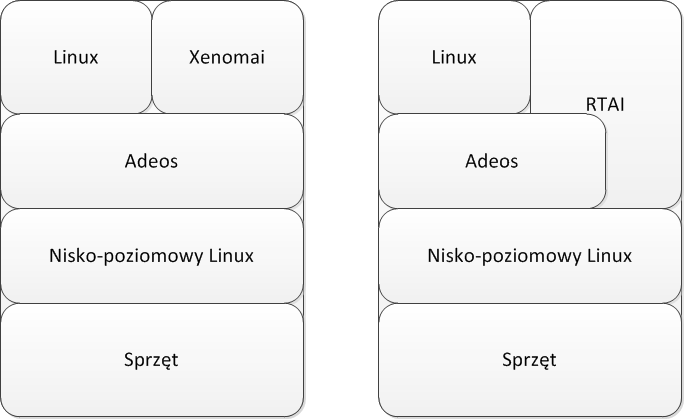
\includegraphics[width=300px]{img/XenomaiRTAI}
\caption{Architektura Xenomai i RTAI}
\label{XenomaiRTAI}
\end{center}
\end{figure}

Propagacja przerwań odbywa się za pośrednictwem kolejki. Kolejka jest łańcuchem (ang. \emph{pipeline}) systemów operacyjnych, które są kolejno budzone w reakcji na otrzymane przerwanie. W przypadku Xenomai jest on umieszczony na początku kolejki i obsługuje przerwania związane z zadaniami czasu rzeczywistego. RTAI, zgodnie ze swoją polityką maksymalnej redukcji opóźnień, samodzielnie przyjmuje przerwania, a kolejki Adeos używa jedynie do dalszej propagacji nieobsłużonych przerwań (\ref{XenomaiRTAI}). 

Warto wspomnieć również o udostępnianej w środowisku Xenomai opcji \emph{skórek RTOS} (ang. \emph{real-time operating system skins}). Pozwalają one na wybór API, z którego będą korzystać uruchamiane w Xenomai aplikacje. Do wyboru są przykładowo skórki VxWorks, co ukazuje tendencje rozwoju w stronę przenośności rozwiązania.

\subsection{Porównanie Linux 2.6, Xenomai, RTAI i VxWorks.}

Z dostępnego w publikacji \cite{pub:Comparison} zestawienia systemów wynika głównie, że w prostym scenariuszu, kiedy znana jest liczba (w tym przypadku wyłącznie jedna) i rodzaj pracujących aplikacji czasu rzeczywistego, system Linux w wersji 2.6 spisuje się zadowalająco w roli systemu o łagodnych ograniczeniach czasowych. W przypadku jądra systemu Linux 2.6 razem z liczbą i stopniem skomplikowania uruchamianych aplikacji rośnie również ilość kodu do przeanalizowania, w celu zapewnienia całkowitego determinizmu operacji, co szybko staje się niepraktyczne.

Interesujący jest dla mnie fakt, że gdy w rolę wchodzi dodatkowo komunikacja sieciowa, systemy \emph{open-source} (RTAI i Xenomai) spisują się znacznie lepiej od VxWorks. Mniejsze opóźnienia są spowodowane wykorzystaniem modułu RTnet, który przebudowuje standardowy stos IP systemu Linux pod kątem deterministycznej pracy.

%%%%%%%%%%%%%%%%%%%%%%%%%%%%

\section{Standardy 802.11 w systemach czasu rzeczywistego.}

Ze względu na swój charakter komunikacja bezprzewodowa jest nieprzewidywalna. Nie jesteśmy w stanie z góry założyć, ze sygnał nie zostanie zakłócony i informacja dotrze do celu. Pocieszający jest fakt, że na przestrzeni lat standard 802.11 podlegał wielu modyfikacjom i poprawkom (np. 802.11e, 802.11n). Część z tych aktualizacji dedykowana była możliwości zastosowania medium bezprzewodowego do komunikacji systemów czasu rzeczywistego. Koncentrują się one na potrzebie zapewnienia takiemu systemowi okien dostępu bezkolizyjnego i nadawaniu priorytetów w ruchu sieciowym. Zabiegi te pozwalają na osadzenie komunikacji systemów czasu rzeczywistego w zakłóconym paśmie transmisyjnym oraz ich koegzystencję z innymi stacjami. 

Niniejszy rozdział poświęcony jest przeglądowi dostępnych rozwinięć standardu 802.11 pod kątem użyteczności w komunikacji systemów czasu rzeczywistego.

\subsection{Problemy w 802.11 MAC - opcja DCF.}

Podstawowa wersja protokołu dostępu do medium (ang. \emph{Distributed Coordination Function}, w skrócie DCF) nie uwzględnia możliwości ustalenia priorytetów. Brak priorytetów na poziomie MAC w oczywisty sposób utrudnia realizację przewidywalnej komunikacji w systemie czasu rzeczywistego. System musiałby konkurować ze wszystkimi innymi stacjami (nawet tymi, które nie są świadome jego istnienia, a więc wprowadzają wyłącznie zakłócenia). 

Dodatkowo, stacje, które przy próbie dostępu napotkały zajęty kanał transmisji, muszą odczekać pewien losowy okres czasu (ang. \emph{Backoff}). Długość okresu oczekiwania obliczana jest jako iloczyn losowej wartości z zakresu od zera do ustalonej długości CW (ang. \emph{Contention Window}) i czasu podróży ramki w łączu (ang. \emph{Slot Time}). Oczywiste jest, że wprowadzenie losowego parametru kłóci się z ideą deterministycznej pracy.

\subsection{802.11 MAC - opcja PCF.}

Część powyżej przedstawionych problemów jest adresowana przez wprowadzenie protokołu dostępu PCF (ang. \emph{Point Coordination Function}). Opcja ta wyróżnia jedną stację (typowo jest to punkt dostępu - AP), która pełni rolę koordynatora komunikacji. Koordynator uzyskuje dostęp do łącza częściej, gdyż jego czas oczekiwania między kolejnymi ramkami jest krótszy. Po uzyskaniu dostępu do łącza koordynator wybiera stację, która może rozpocząć transmisje w oknie bezkolizyjnym. 

W tym przypadku problemem jest fakt, że nadająca stacja może wysłać ramkę arbitralnej długości. Punkt dostępowy rozsyła z okresem TBTT (ang. \emph{Target Beacon Transmission Time}) ramki typu \emph{Beacon} 
porządkujące transmisję danych. Przykładowo w 802.11e ramki \emph{Beacon} zawierają ustawienia parametrów (np. TXOP) i
informują inne stacje o zakończeniu okresu dostępu bezkolizyjnego.
Protokół dostępu PCF nie posiada ograniczeń, które mogłyby powstrzymać stację przed pogwałceniem okresu TBTT. Jest
możliwe, że stacja, która została wybrana przez AP w okresie dostępu bezkolizyjnego rozpocznie przesyłanie zbyt dużych ramek,
których czas przesyłania przekroczy czas okresu TBTT. Przekroczenie czasu TBTT powoduje, że AP opóźni propagację ramek
\emph{Beacon}. Brak możliwości deterministycznego określenia długości trwania okresu dostępu bezkolizyjnego, czy też samego
czasu transmisji pojedynczej stacji w tym okresie powoduje, że obsługa komunikacji systemów czasu rzeczywistego za pomocą
protokołu PCF jest utrudniona.

\subsection{Wsparcie dla QoS w standardzie 802.11e.}

Standard 802.11e wprowadził nowy protokół dostępu EDCA (ang. \emph{Enhanced Distributed Channel Access}). Protokół ten udostępnia 4 klasy priorytetów dla ruchu. System priorytetów zbudowany jest na bazie parametrów odziedziczonych po protokole DCF. 

Każda klasa dostępu posiada własny odstęp międzyramkowy AIFS (ang. \emph{Arbitration Interframe Space}).

Czas \emph{Backoff} nadal wyliczany jest w sposób losowy, ale w tym przypadku jest to wartość z przedziału od zera do górnej granicy, która na wstępie wynosi CWmin. W sytuacji dużej zajętości medium, kiedy stacja natrafia na zajęty kanał to wartość maksymalna jest zwiększana, ale nie wyniesie więcej niż CWmax (CWmin i CWmax są parametrami ustalanymi indywidualnie dla każdej klasy dostępu).

Może dojść do sytuacji, kiedy natężenie ruchu w sieci komunikacyjnej jest na tyle duże, że priorytety nie wystarczają dla zapewnienia odpowiedniej jakości połączenia dla systemu czasu rzeczywistego. W takiej sytuacji możliwe jest użycie parametru TXOP (ang. \emph{Transmission Oportunity}). 

Parametr TXOP pozwala stacji na transmisję serii ramek (ang. \emph{burst}). Po uzyskaniu dostępu do łącza
węzeł może przesyłać kolejne ramki z odstępem SIFS (ang. \emph{short interframe space}) między porcją danych, a
ramką potwierdzenia ACK. TXOP zapewnia bezkolizyjny dostęp do medium jednocześnie ograniczając maksymalny czas 
okresu dostępu bezkolizyjnego dla danej stacji. Jeśli przesyłanie ramki trwałoby dłużej niż czas TXOP to ramka
ta zostanie podzielona, aby zachować jakość usług.

Podsumowując, istnieją 4 parametry podlegające niezależnej regulacji w ramach każdej z klas dostępu:

\begin{itemize}
\item CWmin - minimalna długość losowego składnika czasu \emph{Backoff}.
\item CWmax - maksymalna długość losowego składnika czasu \emph{Backoff}.
\item AIFSN - Składnik odstępu międzyramkowego. 
\item Max TXOP - Maksymalny czas dostępu bezkolizyjnego po uzyskaniu medium.
\end{itemize}

Ostateczna długość \eqref{eq:AIFS} odstępu międzyramkowego AIFS (ang. \emph{Arbitration Inter-frame Spacing}) wyliczana jest poprzez sumowanie czasu SIFS (ang. \emph{Shot Inter-frame Spacing}), który jest wartością stałą, z iloczynem AIFSN (Składnik odstępu międzyramkowego dla danej klasy dostępu) i czasu podróży danych w łączu (ang. \emph{Slot Time}). Czas SIFS jest najkrótszym z dostępnych w specyfikacji odstępów międzyramkowych.    

\begin{figure}
\caption{Wzór na odstęp międzyramkowy.}
\begin{equation} 
\label{eq:AIFS}
AIFS = SIFS + AIFSN * Slot Time 
\end{equation}
\end{figure}

Warto zauważyć, że zmniejszanie czasów oczekiwania rywalizującej stacji umożliwia jej częstszy
dostęp do medium, lecz powoduje również wzrost kolizji na łączu. Wynika z tego, że w celu stworzenia dogodnego środowiska dla pracy systemu czasu rzeczywistego należy ograniczyć liczbę stacji obsługiwaną przez dany punkt dostępowy. W sytuacji osiągnięcia maksimum \emph{AP} nie musi wykonywać już procesu asocjacji. Parametr ten powinien być łatwo dostępny w większości interfejsów obsługi punktów dostępowych (przykładowo w pliku konfiguracyjnym demona \emph{hostapd} służy do tego wartość \emph{max\_num\_sta}).

\subsection{Zastosowanie 802.11e w przykładowym środowisku.}

Standard 802.11e udostępnia następujące klasy dostępu:

\begin{itemize}
\item AC\_VO - klasa dostępu głosowego (najwyższy priorytet)
\item AC\_VI - klasa dostępu wideo
\item AC\_BE - klasa ruchu uprzywilejowanego 
\item AC\_BK - ruch w tle (najniższy priorytet)
\end{itemize}

W tym przypadku system czasu rzeczywistego mógłby korzystać z klasy AC\_VO (\cite{pub:802.11e}). Inne stacje świadome istnienia systemu mogą komunikować się w klasie AC\_BK. Jeśli chodzi o stacje nieświadome istnienia systemu to można dla nich przeznaczyć klasę AC\_BE.

\subsection{Rozwiązania na poziomie oprogramowania Linux.}

Mechanizm QoS (ang. \emph{Quality Of Service}) jest realizowany w jądrze 2.6 w postaci struktury komponentów, z których każdy realizuje pewien podzbiór funkcjonalności związanych z sterowaniem ruchem sieciowym (\cite{pub:QoS}). Główne składniki modułu QoS w systemie Linux to:

\begin{itemize}
\item qdisc - odpowiada za politykę kolejkowania ramek na urządzeniu.
\item class - umożliwia podział pakietów na klasy priorytetów w ramach qdisc.
\item filter - jest elementem odpowiadającym za podział na klasy lub np. upuszczanie ramek.
\end{itemize}

Wstępnie dostępne są dwa elementy qdisc - ingress i root (egress). Główna funkcjonalności skupia się w qdisc'u root, gdyż odpowiada on za kolejkowanie ramek wychodzących ( qdisc ingress umożliwia jedynie np. proste upuszczanie ramek ).

Istnieją dwa typy komponentów qdisc - korzystający z klas (ang. \emph{classfull qdisc}) i nie korzystający z klas (ang. \emph{classless qdisc}). 

Qdisc nie wykorzystujący klas pozwala na realizację prostej polityki kolejkowania typu FIFO (ang. \emph{First-in-first-out}). Standardowo, system Linux do kolejkowania swoich ramek wykorzystuje qdisc typu \emph{pfifo\_fast}, która składa się z trzech kolejek FIFO opróżnianych wedle swojego priorytetu. \emph{Classless qdisc} pozwala na realizację prostej polityki ograniczania częstotliwości ramek. TBF (ang. \emph{Token Bucket Filter}) bazuje na buforze wypełnianym małymi porcjami danych (żetonami), które są konsumowane przez wysyłane ramki.

Qdisc korzystający z klas pozwala na implementację bardzo skomplikowanych struktur drzewiastych (ang. \emph{Hierachical Token Bucket}). Każda klasa może zawierać inne klasy, przy czym w liściach drzewa następuje kształtowanie ruchu (znajdują się tam elementy qdisc). Klasy służą jedynie do odpowiedniego podziału dostępnych żetonów. Zaimplementowano również mechanizm pożyczania. Jeśli klasa dziecko wyczerpała dostępne żetony, to pożycza je od klasy rodzica.

\subsection{Stos IP RTnet.}

RTnet jest nowym stosem IP przeznaczonym dla systemów Xenomai i RTAI. Zastępuje on standardowy stos systemu Linux i wprowadza zmiany istotne z punktu widzenia komunikacji systemów czasu rzeczywistego.

Bufor pakietu \emph{sk\_buff} został zastąpiony przez strukturę \emph{rtskb}, która ma następujące własności:

\begin{itemize}
\item Stały rozmiar (zawsze maksymalny)
\item Pula buforów jest alokowana na początku działania systemu dla każdej warstwy stosu
\item Bufory są przekazywane między warstwami na zasadzie wymiany
\end{itemize}

Wymiana buforów \emph{rtskb} jest konieczna ze względu na potrzebę utrzymania zapasu wskaźników na alokowaną pamięć dostępną w puli danej warstwy stosu.

Inną ważną cechą RTnet jest fakt, że implementacja UDP/IP odbywa się poprzez statyczne przypisanie adresów (nie korzysta z protokołu ARP). Dla pakietów IP przesyłanych we fragmentach potrzebne bufory \emph{rtskb} pobierane są z puli globalnej.

